\documentclass[a4paper]{article}
\usepackage[dutch]{babel}
\usepackage[top=2.5cm, bottom=2.5cm, left=2.6cm, right=1.6cm]{geometry}
\usepackage{graphicx}
\usepackage{fancyhdr}
\usepackage{amsmath,amsthm,amssymb}
\usepackage{textcomp}
\usepackage{float}
\usepackage{lscape}
\usepackage{hyperref}
\usepackage{grffile}

\usepackage[T1]{fontenc}
\usepackage[latin1]{inputenc}
\usepackage{titling}


\setlength{\parindent}{0pt}

\newcommand{\graden}{\ensuremath{\tcdegree}}
\newcommand{\todo}[1]{\marginpar{#1}}

\title{RMI Session 2-3: CarRentalAgency}
\author{Thomas Uyttendaele and Matthias van der Hallen}
\date{2012/11/02}
\setcounter{page}{0}
\setlength{\headheight}{15pt}
\pagestyle{fancy}
\fancyhf{}
\fancyhead[L]{\nouppercase{\thetitle}}
\fancyhead[R]{\nouppercase{\leftmark}}
\fancyfoot[L]{\theauthor}
\fancyfoot[R]{\thepage}

\newtheorem{Stelling}{Stelling}
\newtheorem{Bewijs}{Bewijs}

\begin{document}

\begin{titlepage}

\pagestyle{plain}

\begin{center}
	{\Large Gedistribueerde Systemen}
	
	\vspace{3cm}

	{\Huge \textbf{\thetitle}}
	
	\vspace{5cm}

	{\Large	Thomas Uyttendaele s0215028 \\* Matthias van der Hallen s0219692\\* Burgerlijk ingenieur Eerste Master \\* Computerwetenschappen}
\end{center}

\vspace{8cm}

\begin{center}
	{\Large Begeleiders:\\*
	Prof. S. Walraven\\*}
\end{center}

\vspace{2cm}

\begin{center}
	{\Large \thedate}
\end{center}
 
\end{titlepage}
\renewcommand{\contentsname}{Inhoudstafel}
\tableofcontents
\newpage
\section{Overview Design}
In this section there will be an overview of the most important components and their responsibilities. 
This will all be discussed with the aid of the following \emph{class diagram} \ref{fig:classdiagram}. 
\begin{figure}[hbtp]
\centering
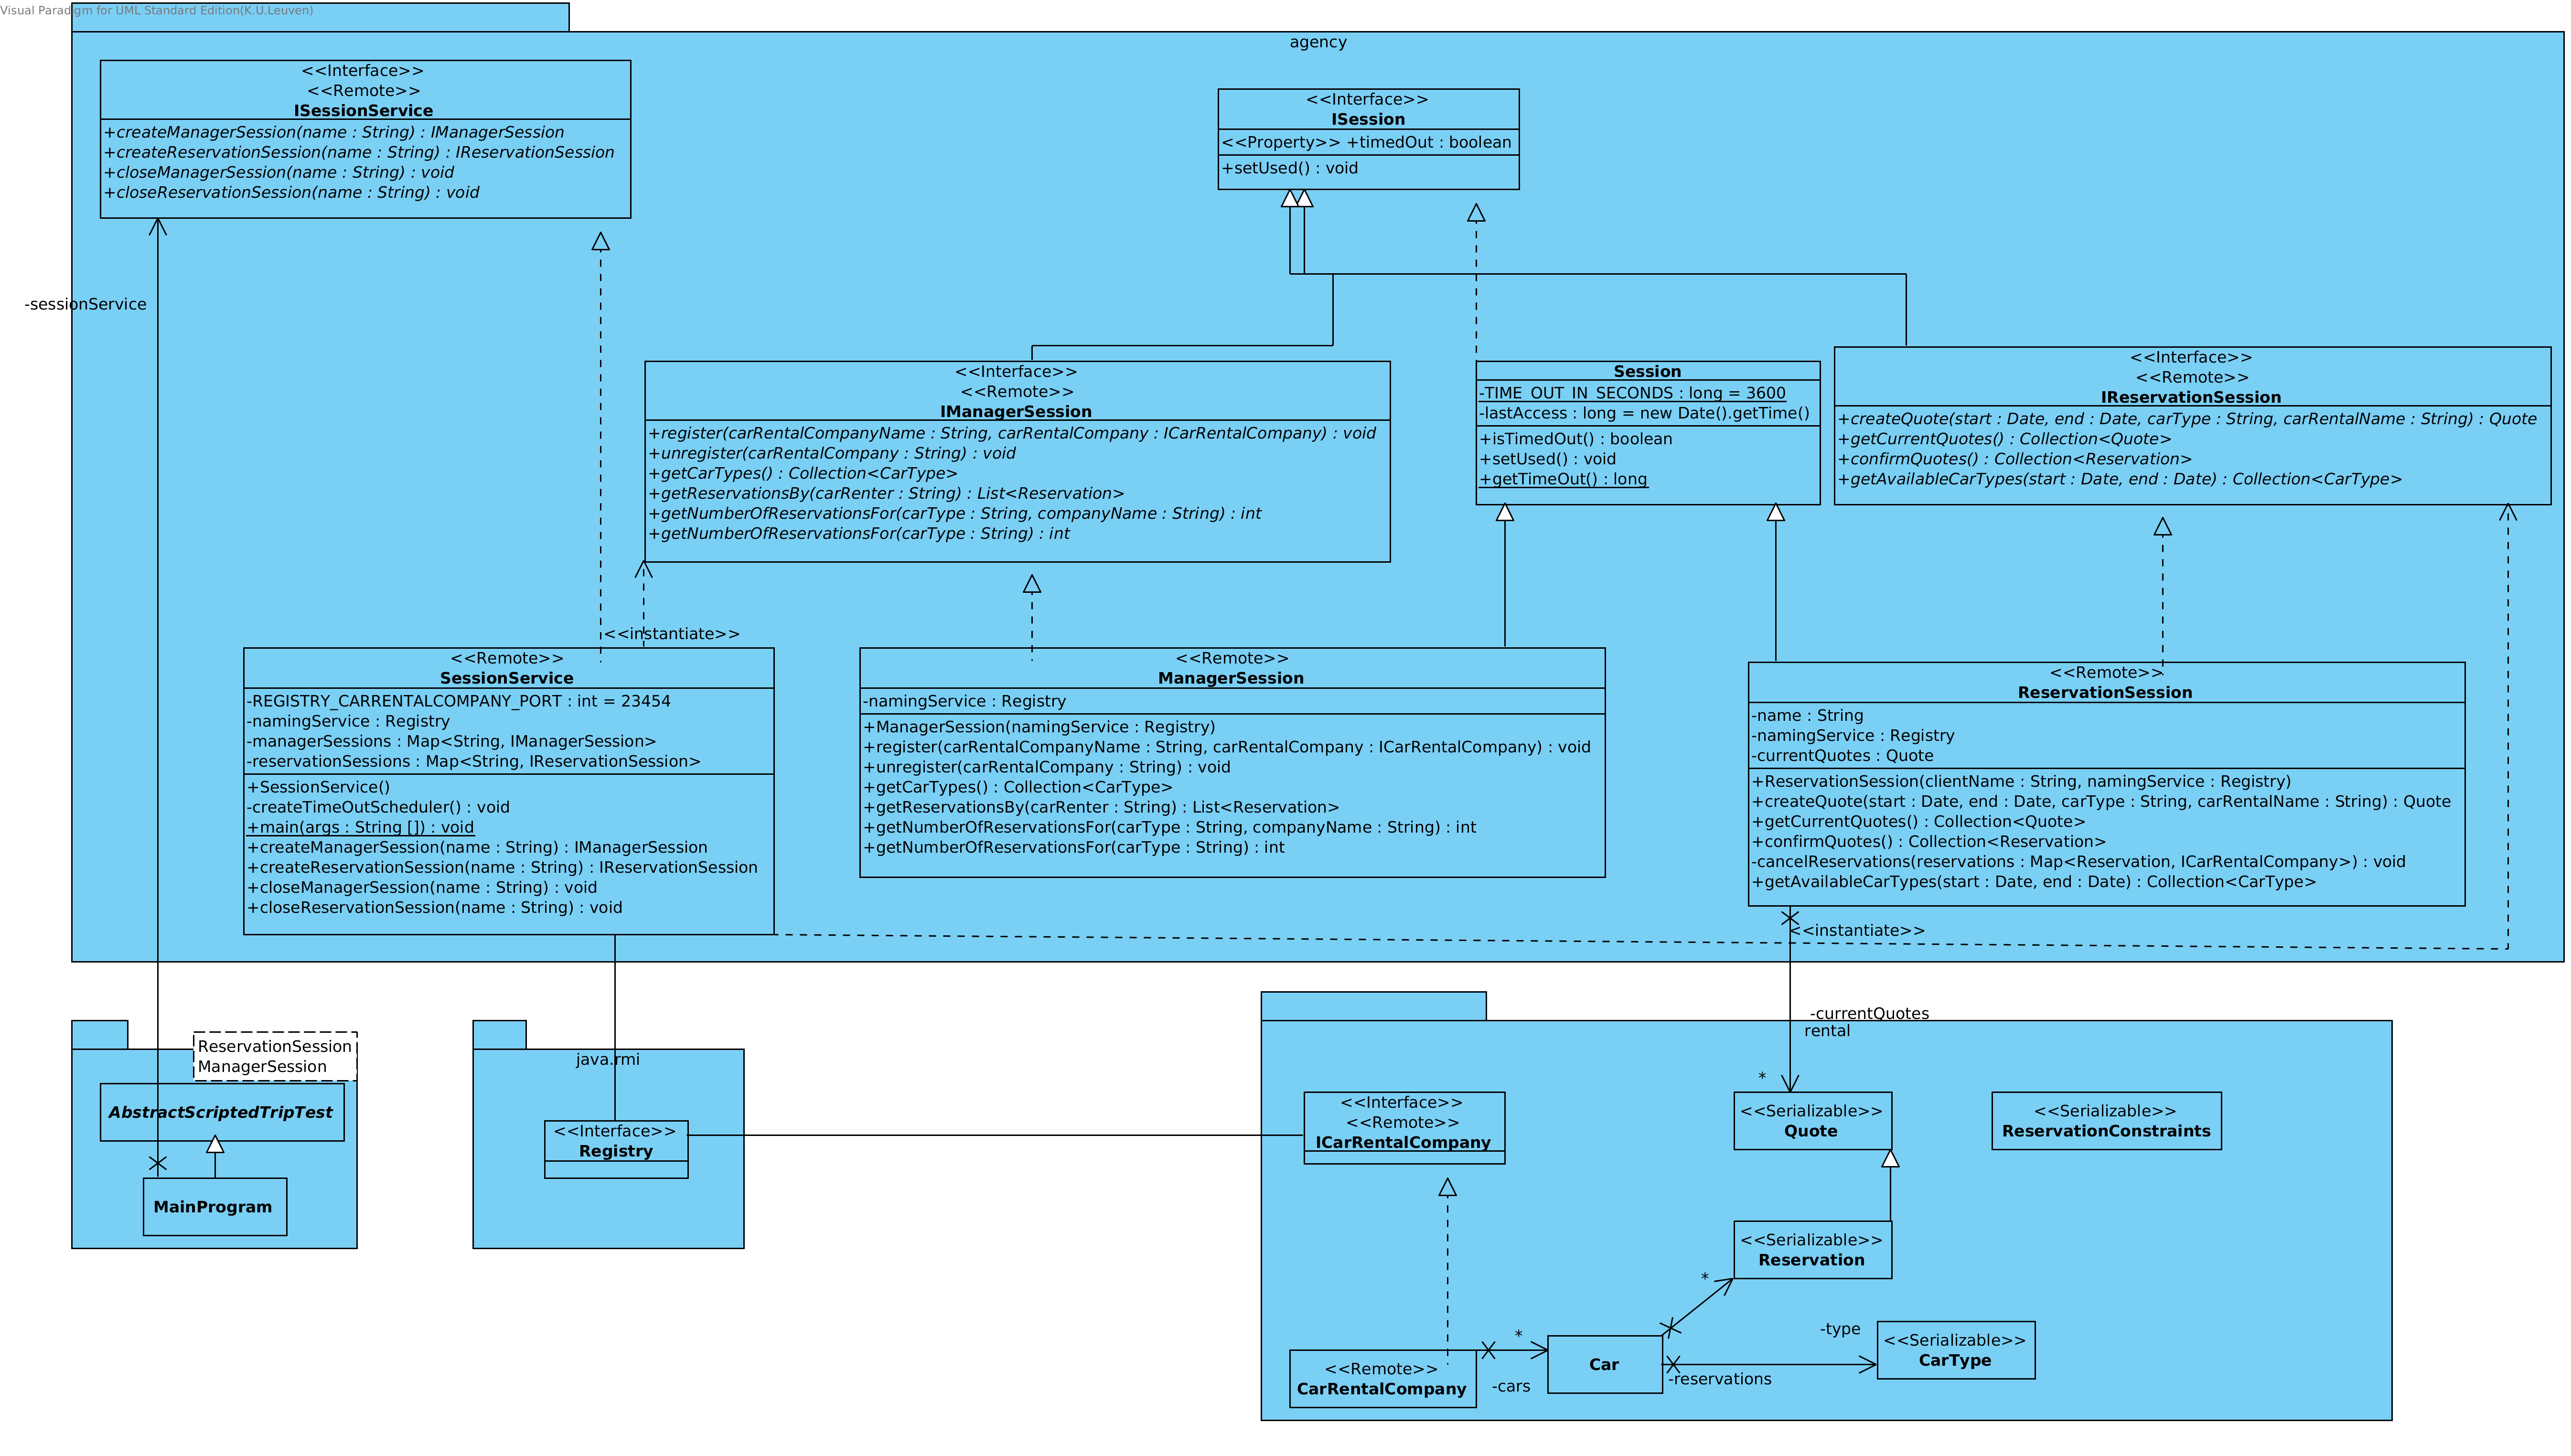
\includegraphics[width=\textwidth]{img/RMI 2-3.png}
\caption{Overview of the design}
\label{fig:classdiagram}
\end{figure}

\subsection{\texttt{SessionService}}
This is the factory class for the creation of new \texttt{Manager}- and \texttt{ReservationSession}s. During initialization, it registers itself at the standard JAVA RMI Registry. \texttt{SessionService} runs on the travel agency server. On this server, it is a stand alone program and it provides the main access point to our agencies service. By holding a link to the CarRentalCompany \texttt{Namingservice}, which is a second JAVA RMI Registry that can run on a different server, it can provide the sessions it creates with access to this naming service.

\texttt{SessionService} is also responsible for the garbage collection. It has a link of all the active sessions and in normal use the sessions should be closed with the \texttt{close...Session}-method. When a session is inactive for more than an hour and not closed by the client, it will automatically be closed by the \texttt{SessionService}.
(In our implementation, for testing purposes, the inactivity timeout is only 3.6 seconds instead of the aforementioned one hour.)

\subsection{\texttt{ManagerSession}}
This class is used by managers to access the agency server and perform actions on this server. They can register and unregister new \texttt{ICarRentalCompany}s at the CarRentalCompanies \texttt{NamingService} which was mentioned before. 

It can also perform various statistics related methods, such as \texttt{getReservationsBy(renter:String)}. 

The normal behaviour of the registration process is given in the following \emph{interaction diagram} \ref{fig:activity_carrentalregistration}.
\begin{figure}[hbtp]
\centering
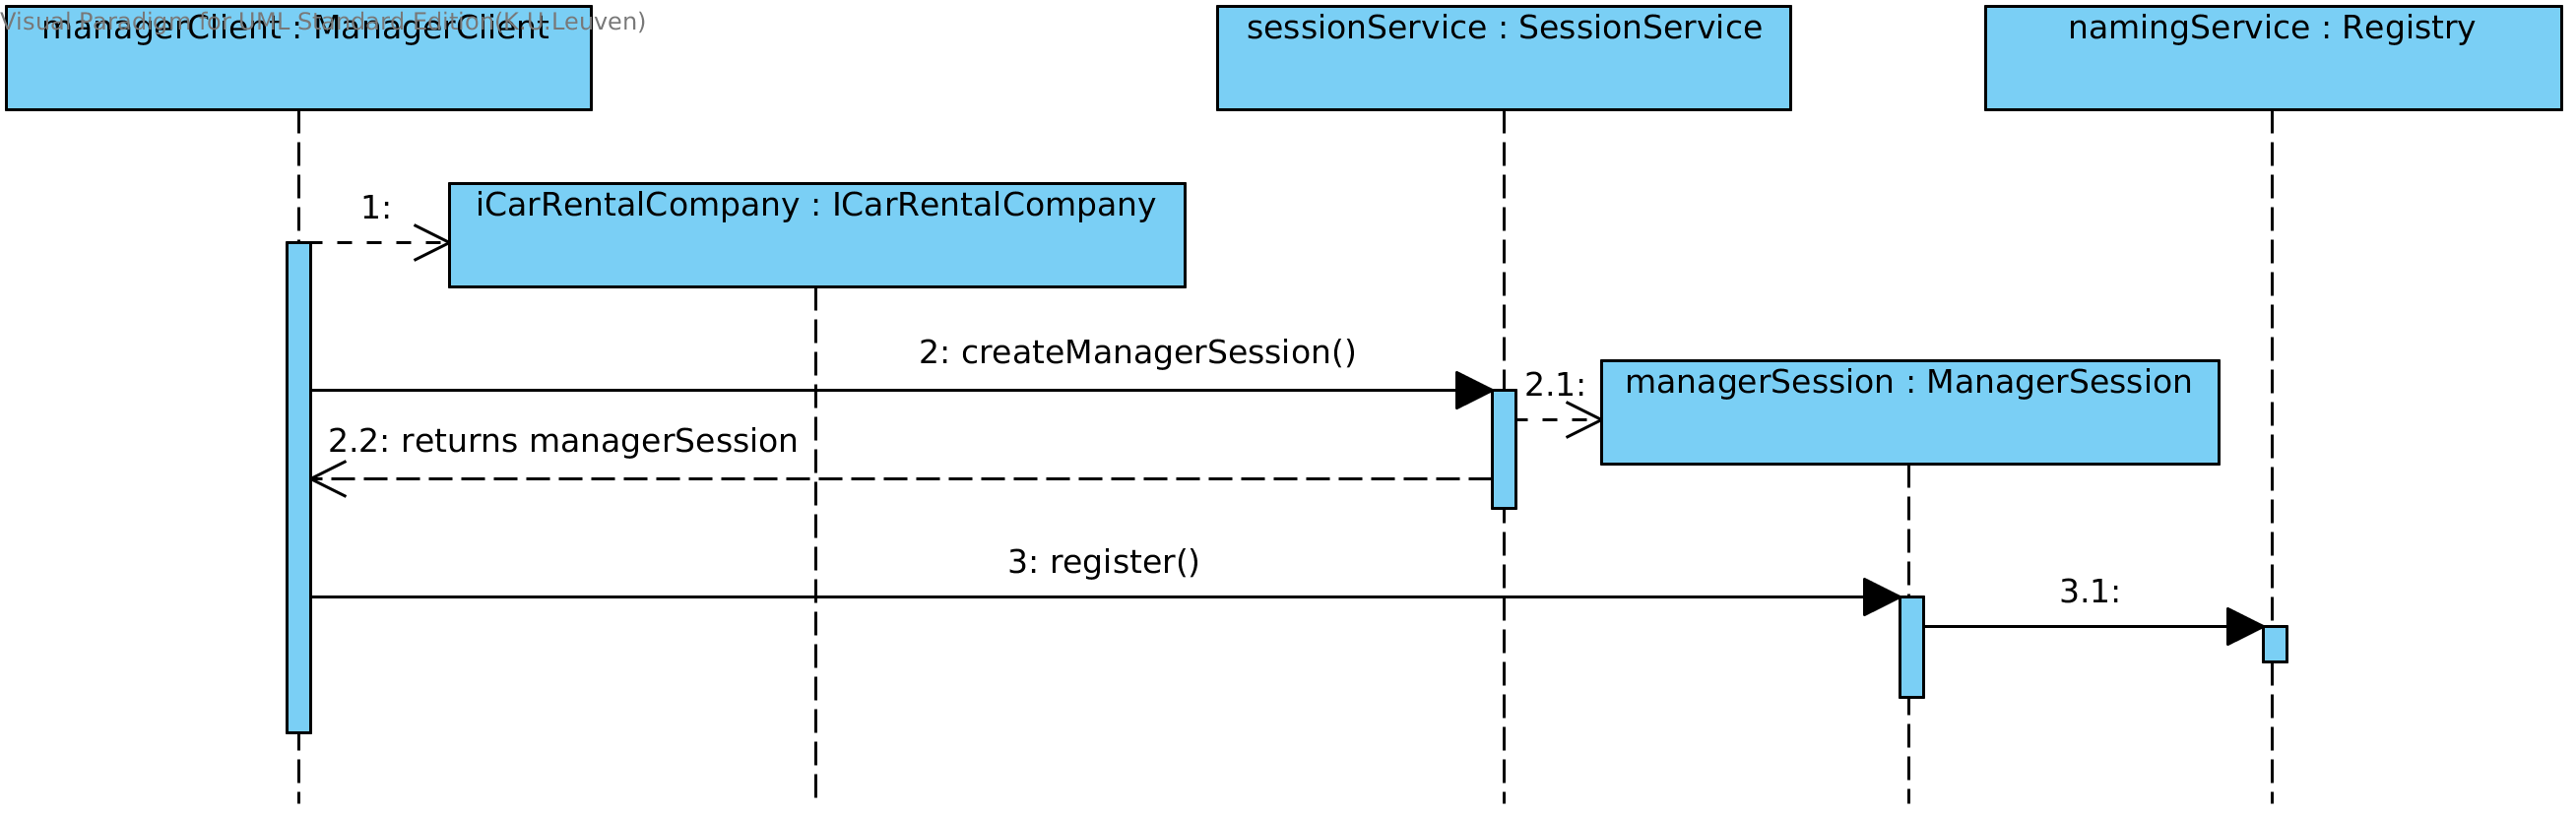
\includegraphics[width=\textwidth]{img/CarRentalCompany registration process.png}
\caption{Interaction diagram of the registration process}
\label{fig:activity_carrentalregistration}
\end{figure}

\subsection{\texttt{ReservationSession}}
This class is used by clients to make reservations on the server. This works in 2 separate steps, to ensure transactional behaviour: first the client creates all the necessary \texttt{Quote}s and afterwards the client can confirm them, at which point they are all reserved, or the entire confirmation fails. 

The transaction behaviour means this process can fail sometimes, when multiple clients are concurrently making reservations. In the first step, by making a \texttt{Quote}, the Car is not yet put aside for the client. This means that if someone else makes a \texttt{Quote} and confirms it in the meantime, then the first clients confirmation will fail if the company doesn't have any identical cars left. In this case, an exception will be thrown. This behaviour is shown in the following  \emph{interaction diagram} \ref{fig:failed_confirmation_diagram}. 

Access to these services are synchronised on the \texttt{NamingService} so only one client at a time can be in these critical sections, for example during a confirmation it won't be possible for others to make a confirmation.
\begin{figure}[hbtp]
\centering
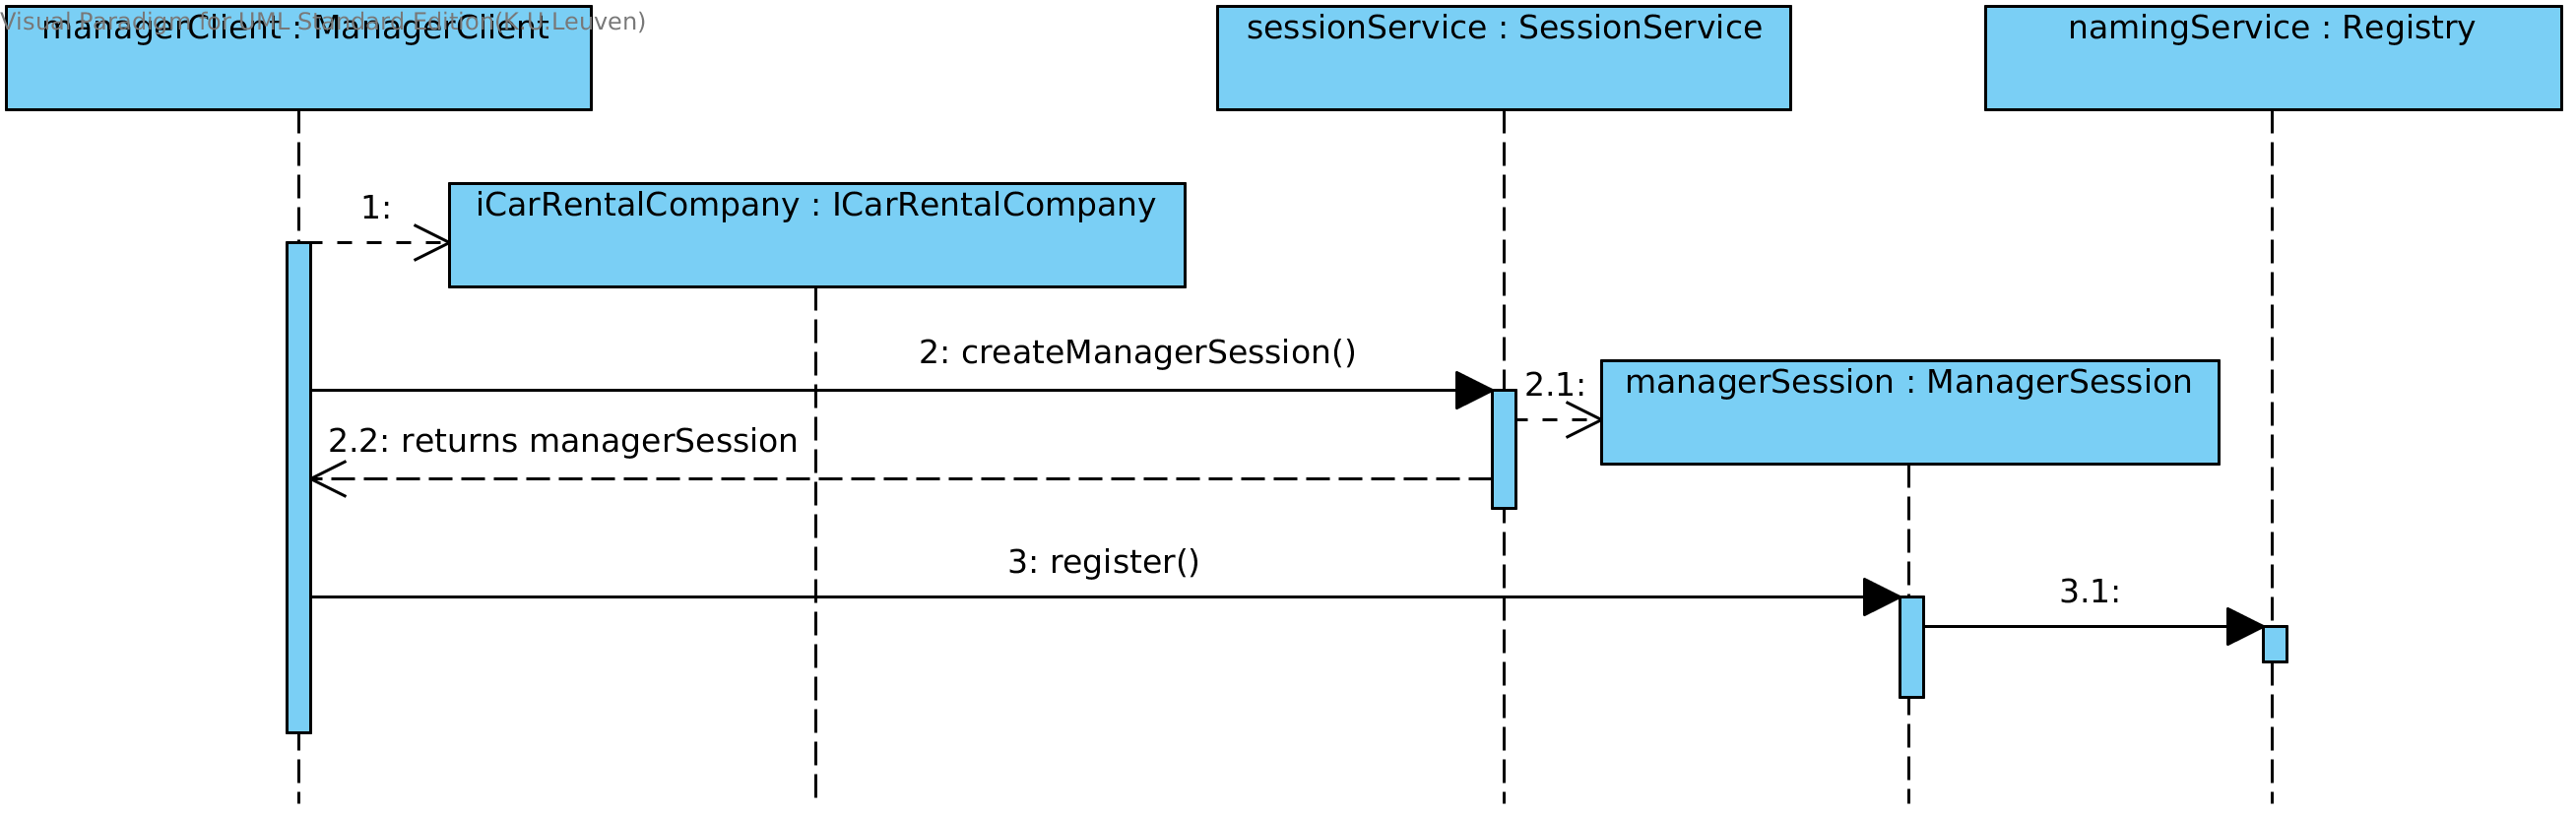
\includegraphics[width=\textwidth]{img/CarRentalCompany registration process.png}
\caption{Interaction diagram of the registration process}
\label{fig:failed_confirmation_diagram}
\end{figure}

\subsection{\texttt{CarRentalCompany}}
This is the regular CarRentalCompany from the first JAVA RMI session. It implements \texttt{Remote} so it could run on the server of the CarRentalCompany itself instead of running on the agency server. 

The rest of the behaviour of this class has stayed the same as in the first JAVA RMI session.

\section{Design Decisions}

\subsection{Remote Access}
As can be found in the \emph{class diagram} (figure \ref{fig:classdiagram}), the following classes are remote: \texttt{ISessionService}, \\ \texttt{IManagerSession}, \texttt{IReservationSession}, \texttt{INamingService} and \texttt{ICarRentalCompany}. These provide an interface to programs running elsewhere, meaning they should be remotely accessible.
The sessions provide a service interface for the client, \texttt{ISessionService} provides a means to create sessions. The \texttt{ICarRentalCompany} is kept separate from all this because it's property of a different company, and the \texttt{INamingService} offers a lookup service where \texttt{ICarRentalCompany}s can be registered.

\texttt{Quote}, \texttt{CarType}, \texttt{ReservationConstraints} and \texttt{ReservationException} are \emph{Serializable} because they are data-classes that never change after initialization, and because they have to be passed from the travel agency server to the client and vice versa. 

\subsection{Deployment of the application}
The deployment of the application is shown on the \emph{deployment diagram} \ref{fig:deployment}.
Most importantly, the \\ \texttt{CarRentalCompany}s run on a different host than the \texttt{SessionService} and the \texttt{NamingService}. This is because they are property of the respective \texttt{CarRentalCompany}s themselves. 

\begin{figure}[hbtp]
\centering
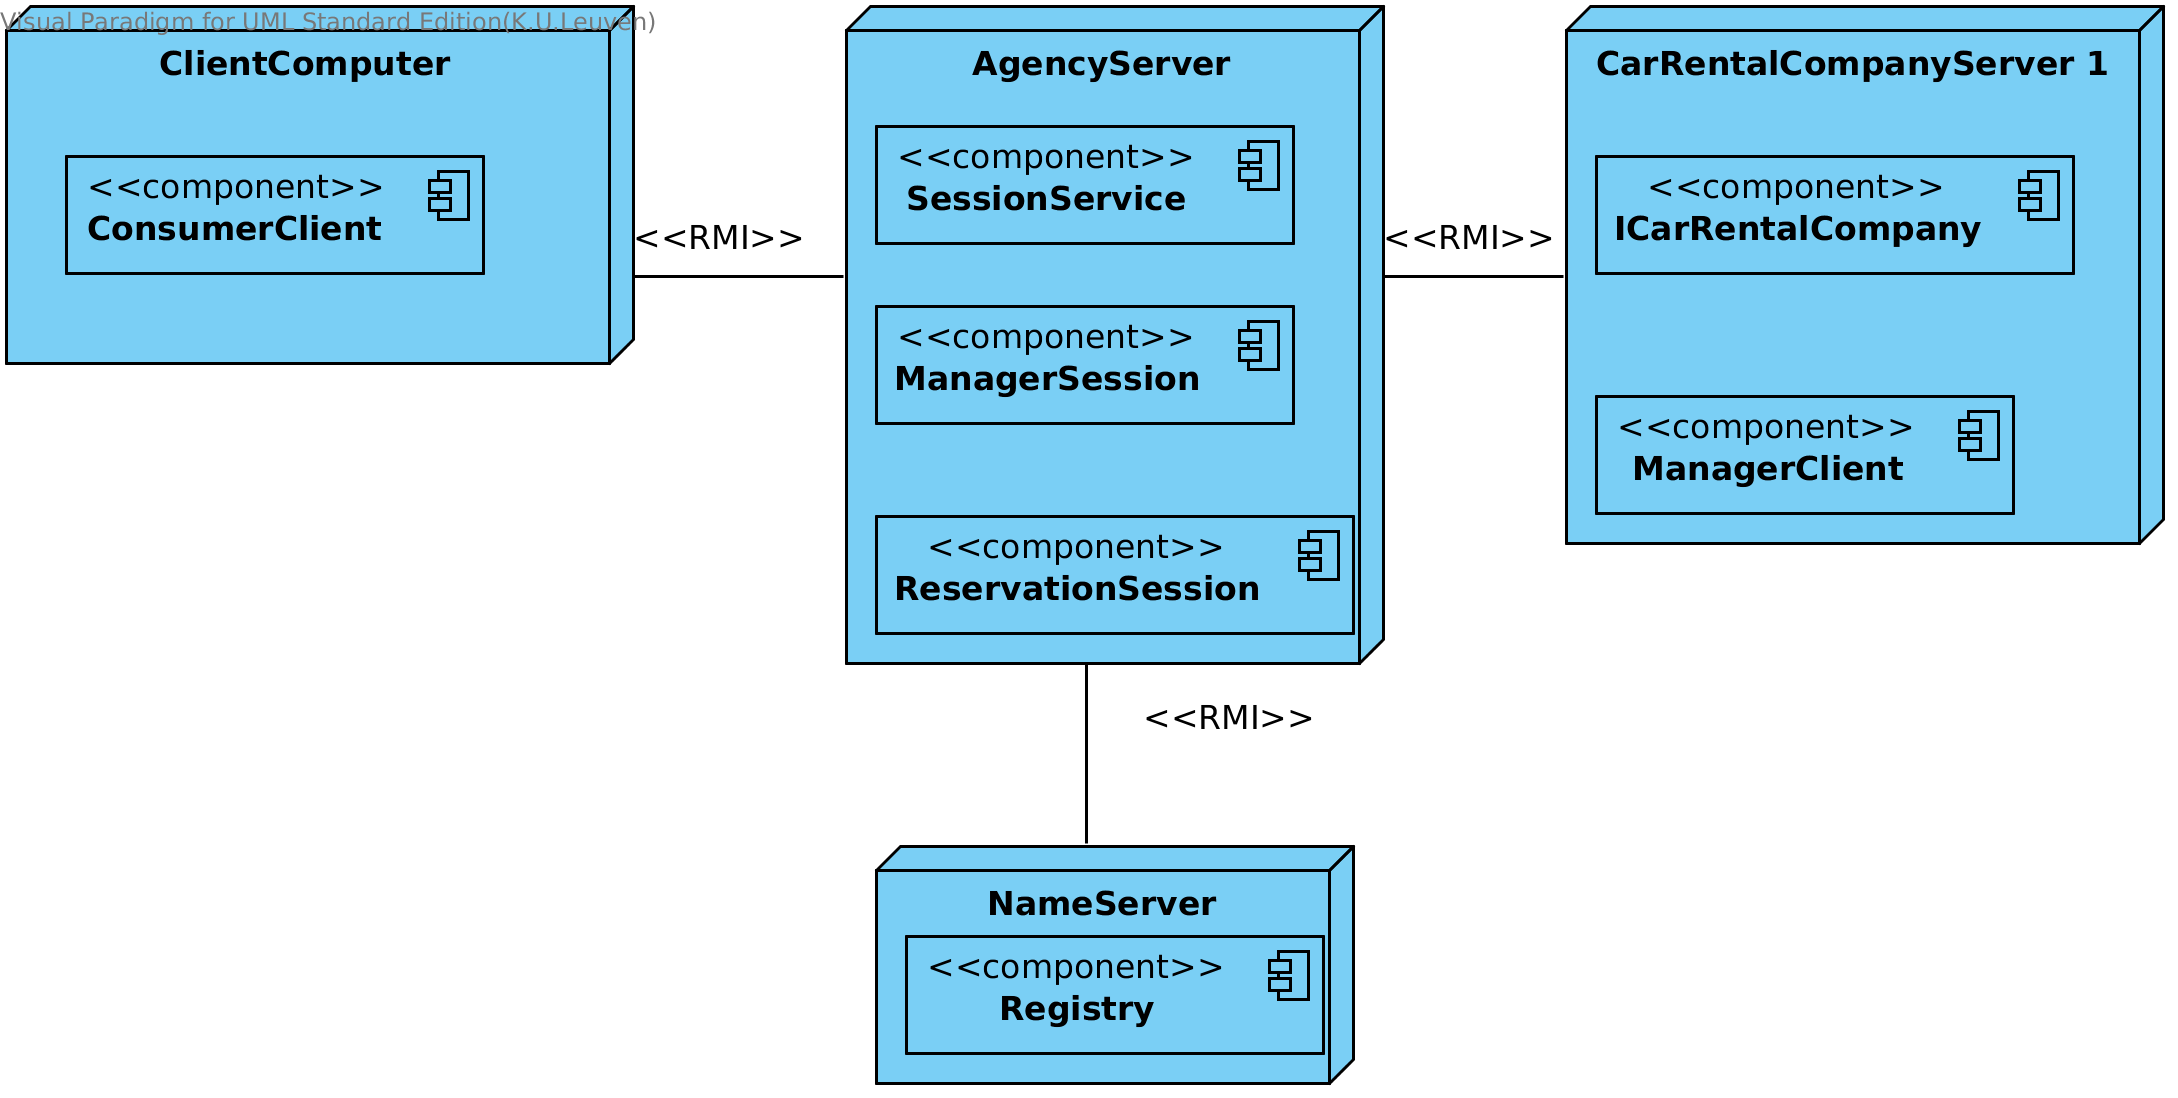
\includegraphics[width=\textwidth]{img/Deployment Diagram.png}
\caption{Deployment of the application}
\label{fig:deployment}
\end{figure}
\subsection{RMI Registration}
The \texttt{NamingService} and the \texttt{SessionService} are registered at their own local JAVA RMI Registry. These are standalone applications running on their own respective servers. \texttt{SessionService} has to know the host and port of the Java RMI Registry that the \texttt{NamingService} bound itself to, so that it can acquire a link to the \texttt{NamingService}. The \texttt{SessionService} is registered on its own local JAVA RMI so that the client can perform a lookup to acquire a hook to the \texttt{SessionService}.

\texttt{CarRentalCompany}s are registered by a \texttt{ManagerSession} at the \texttt{NamingService}, which functions the same way as a JAVA RMI Registry. (It offers registration, unregistration and lookup of objects implementing the Remote interface)

\subsection{Synchronization}
In the \texttt{ReservationSession} class, thread-safety is of utmost importance. When multiple clients are making quotes and confirming them, things could behave unexpectedly. To prevent frustrations and problems, the actions available to this class are performed in a \emph{critical session} by using the JAVA \emph{synchronised} keyword on \texttt{NamingService}. This prevents concurrent users from reserving cars at the same time.

These methods are short, but require remote calls, which means there might be latency from the network which could cause long execution times. This suggests that they are quite prone to becoming a bottleneck. One slight optimization would be to lock on only the companies used in the transaction, instead of all the companies, as in the current implementation. But there are likely other more efficient methods, such as locking on the \texttt{CarType}s (however this is serializable, so extra locking logic is needed) and the corresponding the \texttt{ICarCompany}s involved. That way, more concurrent modifications are possible, but it's also much more difficult to implement, and the synchronization and the locks need more time.

\end{document}